\begin{enumerate}[label=\alph*)]
    \item
        如\cref{figure:5a}所示, 可行域为空, 因此无解.
        \begin{figure}[ht]
            \centering
            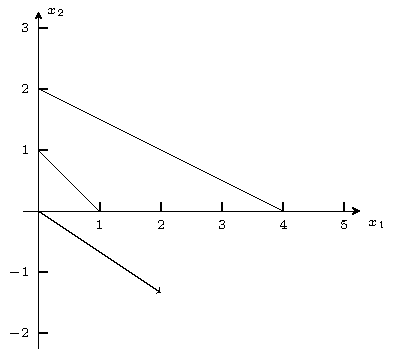
\includegraphics[scale=1.2]{figures/5a.pdf}
            \caption{}
            \label{figure:5a}
        \end{figure}

    \item
        如\cref{figure:5b}所示, 可行域为红色区域.
        $f=-x_1+3x_2$在可行域内可以无限小, 因此无解.
        \begin{figure}[ht]
            \centering
            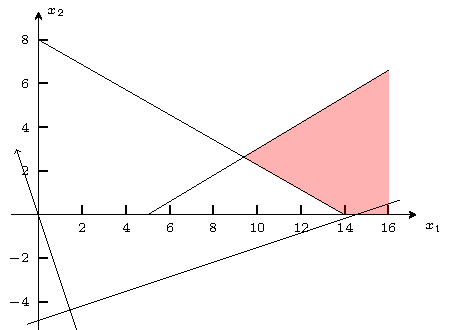
\includegraphics[scale=1.3]{figures/5b.pdf}
            \caption{}
            \label{figure:5b}
        \end{figure}
\end{enumerate}
